\section{interfaz de usuario.}

\begin{figure}[h]
\centering
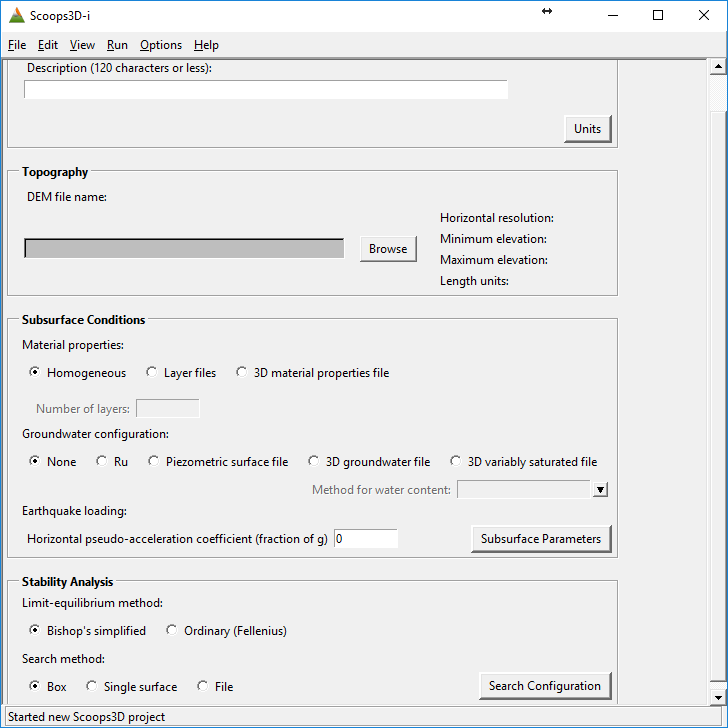
\includegraphics[width=0.5\textwidth]{main_window.PNG}
\caption{Ventana principal de Scoops3D en el sistema operativo Windows. Elavoraci\'on propia.}
\label{fig:Interfaz de usuario}
\end{figure}

La interfaz de usuario principal de Scoops3D  cuenta con 4 secciones principales tituladas Description, Topography, Subsurface Conditions y Stability Analysis. En la secci\'{o}n Description se cuenta con un recuadro de texto en el cual el usuario puede introducir una descripci\'{o}n del proyecto a realizar, adicionalmente, se cuenta con un bot\'{o}n titulado Units (unidades) cuyo funcionamiento se describe a continuaci\'{o}n. \\

\begin{figure}[H]
\centering
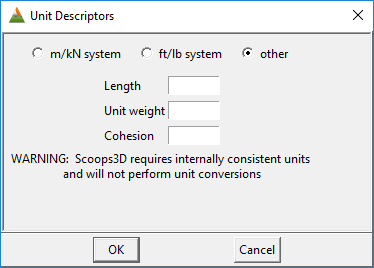
\includegraphics[width=0.5\textwidth]{units_winow.PNG}
\caption{Las unidades seleccionadas pueden modificarse posteriormente.}
\label{unidades}
\end{figure}


En la ventana de selecci\'{o}n de unidades el usuario puede seleccionar las unidades de
esfuerzo a trabajar, o trabajar en sus propias unidades personalizadas. Sin embargo, es
fundamental tener en cuenta que Scoops3D no realiza conversi\'{o}n alguna al momento de su
ejecuci\'{o}n. Por lo cual se debe tener claridad sobre las unidades longitudinales que posee el
DEM as\'{i} como las unidades de \'{a}rea ingresadas en la ventana de b\'{u}squeda de superficie de
falla. Su estructura se ilustra en la figura \ref{unidades}
\\
\begin{figure}[h]
\centering
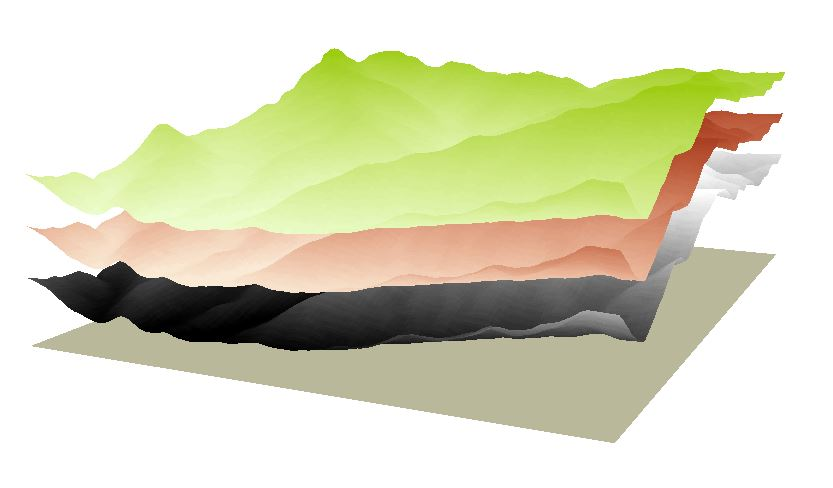
\includegraphics[width=0.9\textwidth]{model.JPG}
\caption{Representci\'on de distintas geolg\'ogicas (verde, rojo, negro). Elaboraci\'on propia.}
\label{geo-units}
\end{figure}


\textbf{Condiciones superficiales.}\\
Scoops3D posee la capacidad de integrar distintas unidades estratigr\'{a}ficas en la simulaci\'{o}n
de superficie de falla. La representaci\'{o}n geom\'{e}trica de dichas unidades se pueden ingresar
a Scoops3D por medio de DEM que representen el techo de cada unidad.
Para usar esta funcionalidad se debe marcar el checkbox layer files en la ventana principal
de Scoops3D.
\\

En caso de ser necesario el uso de varias unidades estratigr\'{a}ficas, es necesario ingresar
los par\'{a}metros de resistencia de cada una de los materiales representados, para lo cual se
hace uso de la ventana de par\'{a}metros subsuperficiales. ilustrada en la figura \ref{fig:parameters}. En esta ventana no es necesario  digital las unidades (MPa) o s\'imbolo alguno para representar los grados del par\'ametro  fi \\

\begin{figure}[H]
\centering
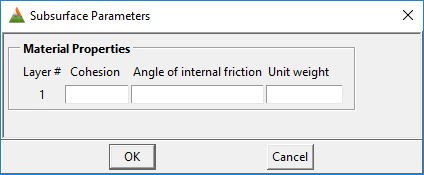
\includegraphics[width=0.8\textwidth]{material_properties_window.PNG}
\caption{Ventana de introducci\'on de p\'arametros de resistencia de unidades geol\'ogicas supbsuperficiales. Elavoraci\'on propia.}
\label{fig:parameters}
\end{figure}


De la misma manera, la cabeza piezom\'{e}trica o nivel fre\'{a}tico se puede representar por
medio de un modelo de elevaci\'{o}n digital como se ilustra en la figura \ref{modelo piezometrico}
\\


\begin{figure}[H]
\centering
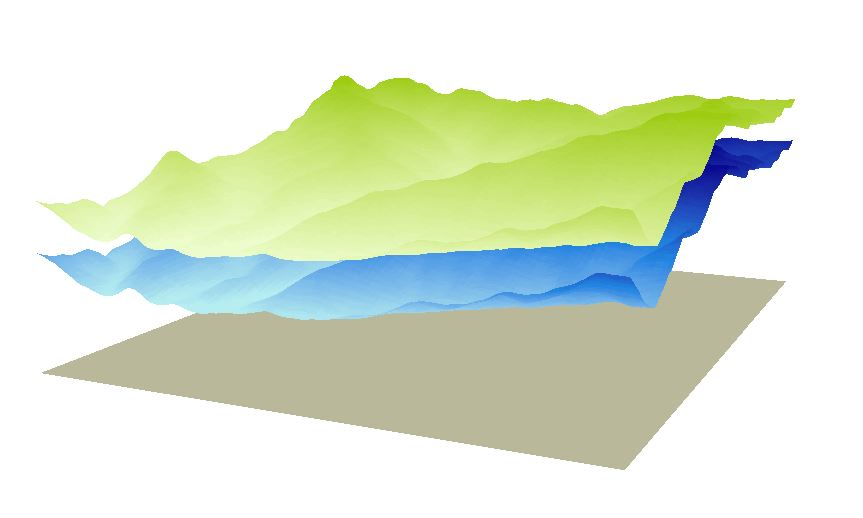
\includegraphics[width=0.8\textwidth]{piezo.JPG}
\caption{Representaci\'on de un nivel priezom\'etrico (azul) como una superficie bajo el DEM superficial (verde). Elaboraci\'on propia.}
\label{modelo piezometrico}
\end{figure}

\textbf{An\'{a}lisis de estabilidad}\\
En el apartado de an\'{a}lisis de estabilidad de la ventana principal de Scoops3D se puede
seleccionar el m\'{e}todo de an\'{a}lisis de estabilidad de laderas que se desea emplear. Las
opciones disponibles son Bishop simplificado y Fellenius.
Asimismo se puede seleccionar el m\'{e}todo de b\'{u}squeda de superficie de falla, las opciones
disponibles son caja, cuyo funcionamiento se detalla en el uso de la ventana search-box.
Superficie espec\'{i}fica, el cual eval\'{u}a la posibilidad de ocurrencia de superficies de Falla
respecto a un \'{u}nico centro de esfera determinado por el usuario. Y por \'{u}ltimo el m\'{e}todo de
b\'usqueda por medio de un archivo de coordenadas XYZ las cuales deber\'an corresponder a
los centros de esfera de falla a evaluar.\par

\textbf{M\'{e}todo de B\'{u}squeda por caja}\\
Inicialmente se definen las dimensiones de la caja de trabajo (figura \ref{searchbox-parameters}) en la cual Scoops3D buscar\'{a}
superficies de Falla. La extensi\'{o}n de dicha caja estar\'{a}n dadas por la altitud m\'{i}nima y
m\'{a}xima del DEM a trabajar y el alcance norte-sur y este-oeste del mismo,el usuario es libre
de modificar estas caracter\'{i}sticas y trabajar con una extensi\'{o}n superior o inferior a las del
DEM.
\begin{figure}[H]
\centering
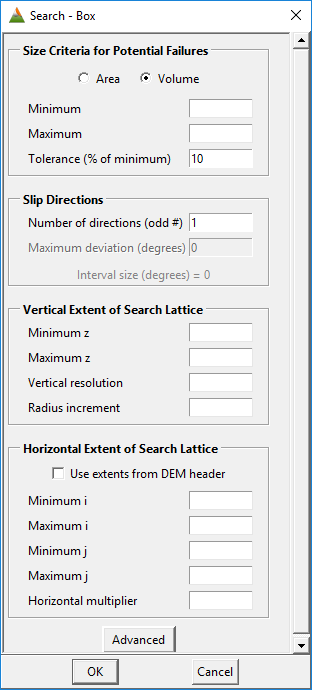
\includegraphics[scale=0.5,keepaspectratio]{search_config_window.PNG}
\caption{Ventana de par\'ametros de la caja de b\'usqueda de superficies de falla, la resoluci\'on de dicha rejilla de b\'usqueda impacta directamente en el tiempo que toma la ejecuci\'on de Scoops3D, este, al ser un programa basado en la arquitectura  bits) no obtiene mayor ventaja con el uso de altas cantidades de memoria RAM ni procesadores con elevado n\'umero de n\'ucleos}
\label{searchbox-parameters}
\end{figure}

